\documentclass[11pt,a4paper]{article}
\usepackage[utf8]{inputenc}\usepackage[T1]{fontenc}\usepackage[spanish]{babel}
\usepackage[margin=2cm]{geometry}\usepackage{graphicx,booktabs,hyperref,amsmath}
\hypersetup{colorlinks=true,urlcolor=blue}\setlength{\parindent}{0pt}\setlength{\parskip}{6pt}
\begin{document}
\begin{center}{\Large Precisión y trabajo con calidad común}\\[4pt]Exploración OMS, 15 de octubre de 2026\end{center}
\textbf{Resultado.} Con cada política fija, cambiar solo el presupuesto de aceptación no cambia ninguna primera llegada. La calidad del objetivo determina la entrega. Recalcular factores con otro presupuesto sí puede cambiar la búsqueda. El contrato exigente gana al conjunto de controles en 3/27 comparaciones, concentradas en un modelo, y pierde en otros. No aparece una ventaja general ni un intercambio práctico precisión/trabajo; OMS permanece sin cambios.

\textbf{Pregunta.} Medir cuánto trabajo hace falta para alcanzar simultáneamente
un presupuesto de precisión y un costo comparable, frente a controles fuertes.
Una parada rápida con costo inaceptable no es una mejora.

\textbf{Diseño.} Tres modelos SG--Ter--Mer de 360 períodos e integralidad
original: 001,022,046, posiciones 1,3,6 del banco limpio anterior. Son conocidos,
no validación en modelos nuevos. 90 brazos; 63 llamadas MILP reales tras
deduplicar; semillas 401,409,419. Gurobi 13.0.2, cuatro hilos, presolve y escalado
internos automáticos, IntegralityFocus=1, tolerancia entera común 1e-9, primal
1e-6 (Tight: 1e-9), gap 0.1\%, 15 s/16 unidades de trabajo. Resoluciones
secuenciales, sin starts, desde los Base.lp archivados. No se usa ni cambia el
generador. Se guardan 1093 candidatos, incluidos los que no mejoran incumbente.

GM, Ruiz y L2 usan potencias de dos dentro de [1e-9,1e9], sin banda identidad.
Todos los productos son exactamente proporcionales; no hay escalado de columnas.
Budget aplica el mismo candidato L2 y exige $\epsilon/\alpha+E\leq\delta$, con
$E=10^{-9}\sum_{j\text{ entero}}|a_{ij}|$. El exigente cambia 1440 factores
de activación por modelo. Referencia/permisivo coinciden con L2. GCD examina
1080 filas enteras por modelo, ya primitivas: coincide con Base; no se aplica
redondeo del RHS a filas con variables continuas.

\textbf{Calidad y precisión.} Se obtiene antes un testigo racional factible por
modelo mediante LP de un patrón conocido, verificando Base. No es un óptimo.
La aspiración común es $C\leq U_{ref}+.01\max(1,|U_{ref}|)$, con referencia
offline declarada, nunca suministrada como Start. Presupuestos (MW,m$^3$):
(.01,100), (.1,1000), (1,10000); objetivos numéricos, no estándares operativos.
Incluyen potencia, envolventes, balances y activaciones, con sus unidades.
Se redondean enteros y se comprueban todas las filas: las otras tienen criterio
auxiliar $10^{-8}\max(1,|b_i|)$; cotas, $10^{-6}$. Costos y residuos se evalúan
exactamente. Alinear denominadores dyádicos para usar enteros no se reclama novedoso.

\newpage
\textbf{Trabajo hasta la precisión exigente y calidad común.}
\begin{center}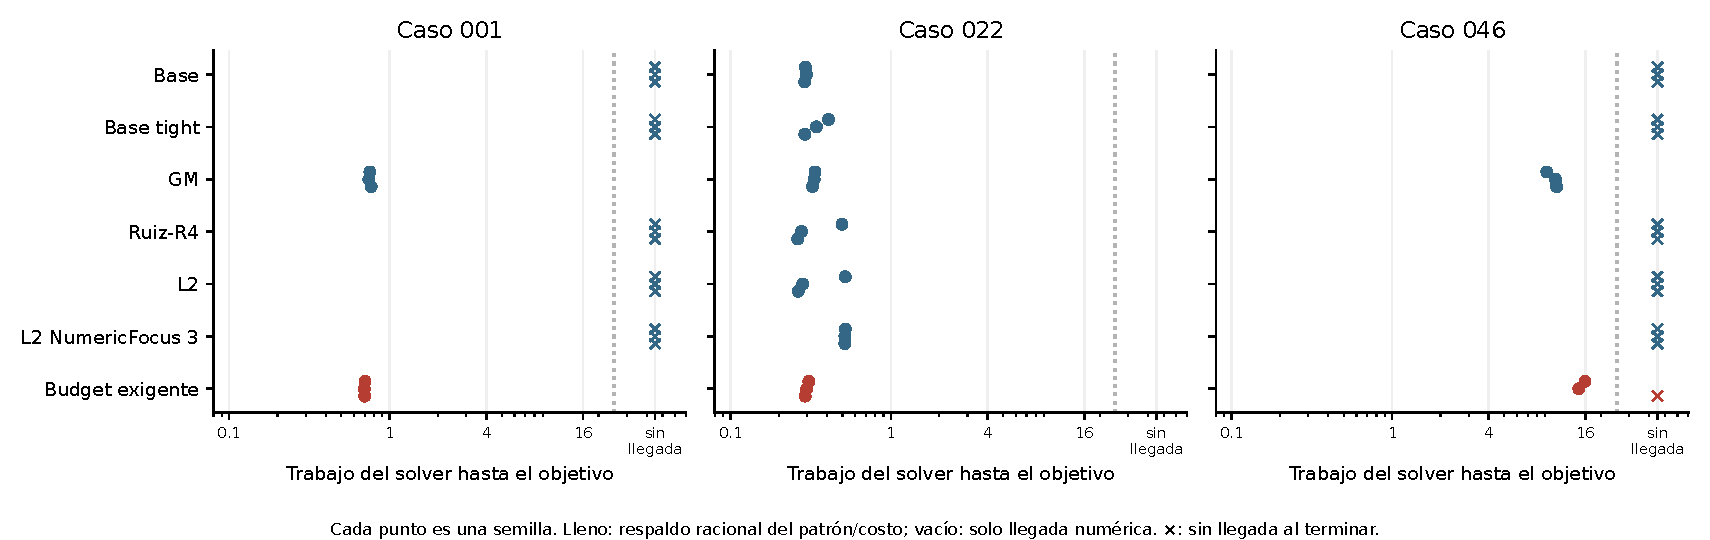
\includegraphics[width=\textwidth]{work-to-target.pdf}\end{center}
Cada punto es una semilla; lleno: respaldo racional del patrón/costo; vacío:
solo llegada numérica. Una cruz significa que no hubo llegada al terminar y su
posición es categórica: no implica haber consumido ese trabajo. Las medianas y
todos los estados/costos figuran en RESULTADOS.md y los CSV.

\begin{center}\small\begin{tabular}{llrrr}\toprule
Caso & Precisión & Llega & Gana controles & Con respaldo\\\midrule
001 & Exigente & 3/3 & 3/3 & 3/3 \\
001 & Referencia & 0/3 & 0/3 & 0/3 \\
001 & Permisivo & 0/3 & 0/3 & 0/3 \\
022 & Exigente & 3/3 & 0/3 & 0/3 \\
022 & Referencia & 3/3 & 0/3 & 0/3 \\
022 & Permisivo & 3/3 & 0/3 & 0/3 \\
046 & Exigente & 2/3 & 0/3 & 0/3 \\
046 & Referencia & 0/3 & 0/3 & 0/3 \\
046 & Permisivo & 0/3 & 0/3 & 0/3 \\
\bottomrule\end{tabular}\end{center}
La política Budget corresponde a la precisión solicitada. Ganar significa menor
trabajo que todos Base, Tight, GM, Ruiz, L2 y L2-NumericFocus del mismo caso y
semilla. El mejor control es una envolvente retrospectiva, no un selector
operativo gratuito. Referencia/permisivo reutilizan L2.

\newpage
\textbf{Respaldo posterior.} Se toma la primera llegada de cada brazo/escenario,
se deduplica por patrón y se intenta un LP racional original por patrón,
sin reemplazar resultados adversos. 25 patrones; 25 llamadas LP
posteriores. Un primal exacto del mismo patrón con $U\leq C_{cap}$ respalda la
calidad; además se exige $U\leq C+.01\max(1,|U|)$ para respaldar el costo nominal.
No es factibilidad exacta del punto flotante original ni óptimo global MILP.
Los desconocidos permanecen como tales. El replay comprueba referencias,
testigos y los residuos mediante un algoritmo independiente de exponentes por
fila y un parser completo de los Base.lp originales.

2 cotas inferiores nativas exceden un testigo factible previo. Se
conservan esas contradicciones. No se valida una cota por no refutarla y no se
usa el gap reportado como prueba del objetivo común.

\textbf{Costo.} La adquisición de referencias es offline y el respaldo posterior
también está fuera de la frontera nativa. La selección se ejecutó y midió por
corrida; se registran construcción, captura, optimización, persistencia y
verificación. Primera llegada se mide retrospectivamente, sin detener ni
alterar el solver. Menor trabajo nativo no implica menor tiempo de un controlador
online, no evaluado aquí. No se suman tiempos de distintos problemas como si
midieran una aceleración a calidad fija.

\textbf{Decisión.} Con cada política fija, cambiar solo el presupuesto de aceptación no cambia ninguna primera llegada. La calidad del objetivo determina la entrega. Recalcular factores con otro presupuesto sí puede cambiar la búsqueda. El contrato exigente gana al conjunto de controles en 3/27 comparaciones, concentradas en un modelo, y pierde en otros. No aparece una ventaja general ni un intercambio práctico precisión/trabajo; OMS permanece sin cambios.

Tres modelos de una familia y tres semillas no prueban generalidad ni efectos
en otro solver. Diferencias de residuos muy inferiores a lo solicitado no
aportan utilidad por sí solas. Los ocho paquetes previos y OMS v1.3.5 se
preservan por SHA256. El diagnóstico LP--DW y los límites conjuntos del
escalamiento siguen pendientes.

\textbf{Fuentes y reproducción.} README.md, PROTOCOL.md, registros originales,
certificados y manifiesto acompañan esta nota. El replay no llama a solvers;
las corridas nuevas requieren Gurobi y los certificados, SoPlex/GMP.
Documentación primaria: \href{https://docs.gurobi.com/projects/optimizer/en/current/reference/numericcodes/callbacks.html}{callbacks 63OL de Gurobi},
\href{https://docs.gurobi.com/projects/optimizer/en/current/concepts/numericguide/numeric_parameters.html}{parámetros numéricos}
y \href{https://soplex.zib.de/doc/html/EXACT.php}{SoPlex exacto}.
\end{document}
